\input{../../../.preambles/02-lab_work}
\newgeometry{top=1.5cm, bottom=1.5cm, left=1cm, right=1cm}
\usepackage{epstopdf}
\begin{document}
    \begin{table}[h!]
        \center
        \begin{tabular}{|C{.5}|C{.2}|C{.25}|}
            \hline
            \multicolumn{1}{|c|}{\multirow{4}{*}{Лабораторная работа № 3}} &
            Студент, группа & {{ student }}, Ф-369 \\ \cline{2-3}
            & Дата выполнения & 16.02.2013 \\ \cline{2-3}
            & Подпись &  \\ \cline{2-3}
            Прохождение гамма-излучения через вещество & Дата отчёта & \\ \cline{2-3}
            & Оценка &  \\ \cline{2-3}
            & Подпись &  \\ \hline
        \end{tabular}
    \end{table}

    \emph{Цель работы:} исследовать зависимость линейного коэффициента
    поглощения от материала, через который проходит пучок, а также от величины
    энергии налетающего гамма-кванта.

    \subsection{Вольфрам}
    \begin{table}[h!]
        \center
        \caption{Результаты эксперимента для вольфрама}
        \begin{tabular}{|C{.11}|C{.14}||C{.13}|*{6}{C{.06}|}} \hline
            Энергия кванта, МэВ & Коэффициент линейного поглощения \( \tau \)
            & Толщина \( x \),~см & 1,0 & 2,0 & 3,0 & 4,0 & 5,0 & 6,0 \\ \hline
            \multirow{2}{*}{10,0} & \multirow{2}{*}{0,895} & \( I(l)/I(0) \) &
            0,427 & 0,164 & 0,065 & 0,027 & 0,011 & 0,005 \\ \cline{3-9}
            & & \( \ln\bigl(I(l)/I(0)\bigr) \) &
            0,370 & 0,785 & 1,187 & 1,569 & 1,959 & 2,301 \\ \hline
            \multirow{2}{*}{8,0} & \multirow{2}{*}{0,850} & \( I(l)/I(0) \) &
            0,430 & 0,180 & 0,080 & 0,032 & 0,015 & 0,006 \\ \cline{3-9}
            & & \( \ln\bigl(I(l)/I(0)\bigr) \) &
            0,367 & 0,745 & 1,097 & 1,495 & 1,824 & 2,222 \\ \hline
        \end{tabular}
    \end{table}
    
    \begin{figure}[h!]
        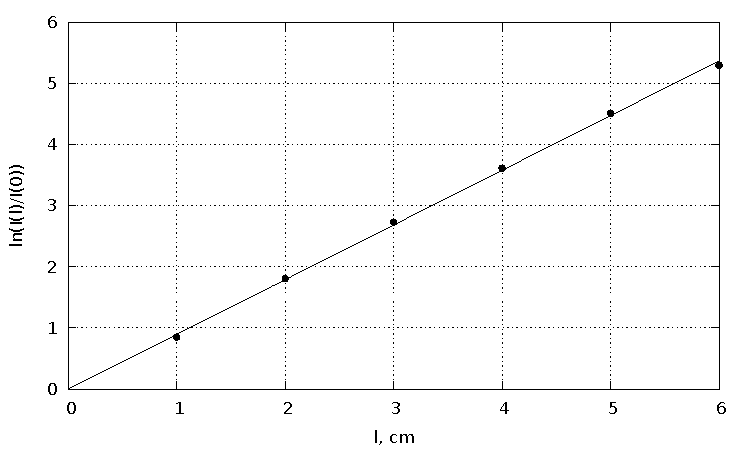
\includegraphics[width=.47\textwidth]{w-10} \hfill
        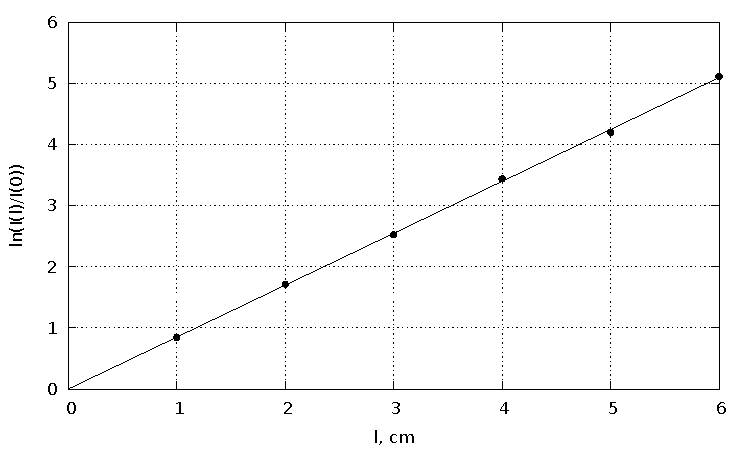
\includegraphics[width=.47\textwidth]{w-8}
        \parbox{.47\textwidth}{\caption{При энергии кванта в 10,0 МэВ}} \hfill
        \parbox{.47\textwidth}{\caption{При энергии кванта в 8,0 МэВ}}
    \end{figure}
    
    \pagebreak
    
    \subsection{Бетон}
    \begin{table}[h!]
        \center
        \caption{Результаты эксперимента для бетона}
        \begin{tabular}{|C{.11}|C{.14}||C{.13}|*{6}{C{.06}|}} \hline
            Энергия кванта, МэВ & Коэффициент линейного поглощения \( \tau \)
            & Толщина \( x \),~см & 1,0 & 2,0 & 3,0 & 4,0 & 5,0 & 6,0 \\ \hline
            \multirow{2}{*}{1,5} & \multirow{2}{*}{0,122} & \( I(l)/I(0) \) &
            0,895 & 0,773 & 0,680 & 0,594 & 0,555 & 0,492 \\ \cline{3-9}
            & & \( \ln\bigl(I(l)/I(0)\bigr) \) &
            0,048 & 0,112 & 0,167 & 0,226 & 0,256 & 0,308 \\ \hline
            \multirow{2}{*}{3,0} & \multirow{2}{*}{0,080} & \( I(l)/I(0) \) &
            0,949 & 0,811 & 0,784 & 0,721 & 0,679 & 0,617 \\ \cline{3-9}
            & & \( \ln\bigl(I(l)/I(0)\bigr) \) &
            0,023 & 0,091 & 0,106 & 0,142 & 0,168 & 0,210 \\ \hline
        \end{tabular}
    \end{table}
    
    \begin{figure}[h!]
        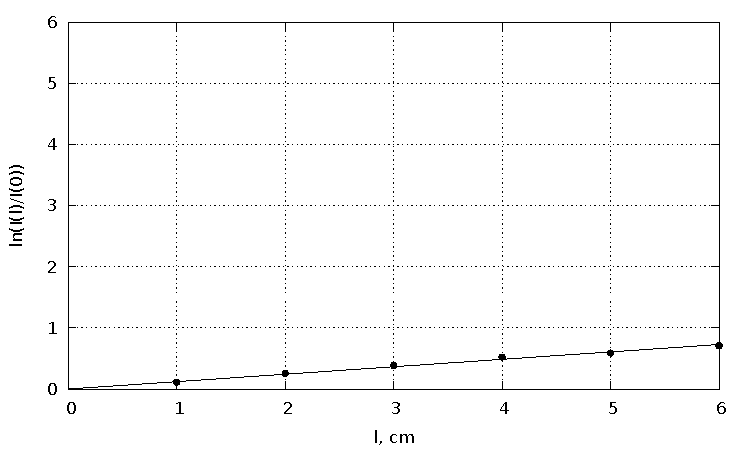
\includegraphics[width=.47\textwidth]{c-1_5} \hfill
        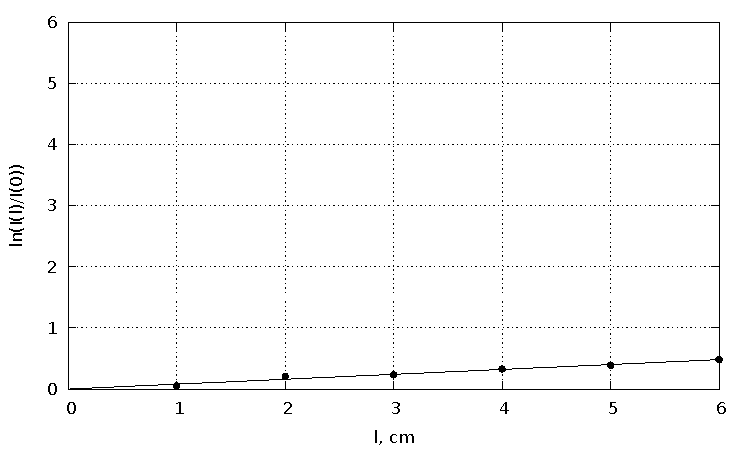
\includegraphics[width=.47\textwidth]{c-3}
        \parbox{.47\textwidth}{\caption{При энергии кванта в 1,5 МэВ}} \hfill
        \parbox{.47\textwidth}{\caption{При энергии кванта в 3,0 МэВ}}
    \end{figure}
    
    \vspace*{-2em}

    \subsection{Фосфор}
    \begin{table}[h!]
        \center
        \caption{Результаты эксперимента для фосфора}
        \begin{tabular}{|C{.11}|C{.14}||C{.13}|*{6}{C{.06}|}} \hline
            Энергия кванта, МэВ & Коэффициент линейного поглощения \( \tau \)
            & Толщина \( x \),~см & 1,0 & 2,0 & 3,0 & 4,0 & 5,0 & 6,0 \\ \hline
            \multirow{2}{*}{0,15} & \multirow{2}{*}{0,250} & \( I(l)/I(0) \) &
            0,747 & 0,606 & 0,454 & 0,357 & 0,284 & 0,237 \\ \cline{3-9}
            & & \( \ln\bigl(I(l)/I(0)\bigr) \) &
            0,127 & 0,217 & 0,343 & 0,447 & 0,547 & 0,625 \\ \hline
            \multirow{2}{*}{0,8} & \multirow{2}{*}{0,125} & \( I(l)/I(0) \) &
            0,853 & 0,784 & 0,706 & 0,584 & 0,520 & 0,483 \\ \cline{3-9}
            & & \( \ln\bigl(I(l)/I(0)\bigr) \) &
            0,069 & 0,106 & 0,151 & 0,234 & 0,284 & 0,316 \\ \hline
        \end{tabular}
    \end{table}
    
    \begin{figure}[h!]
        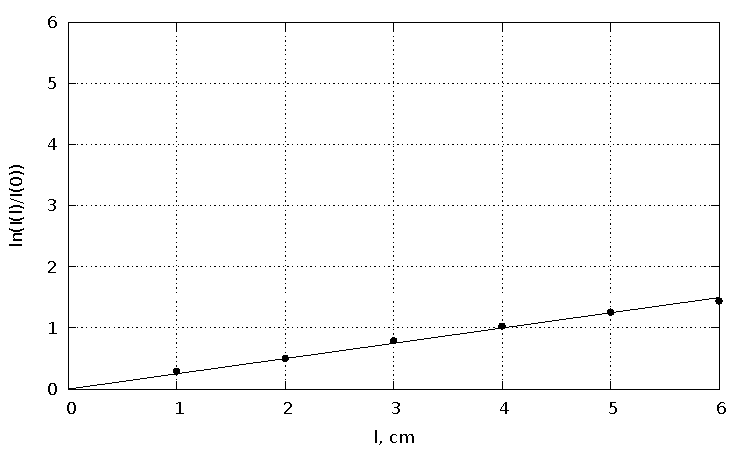
\includegraphics[width=.47\textwidth]{p-0_15} \hfill
        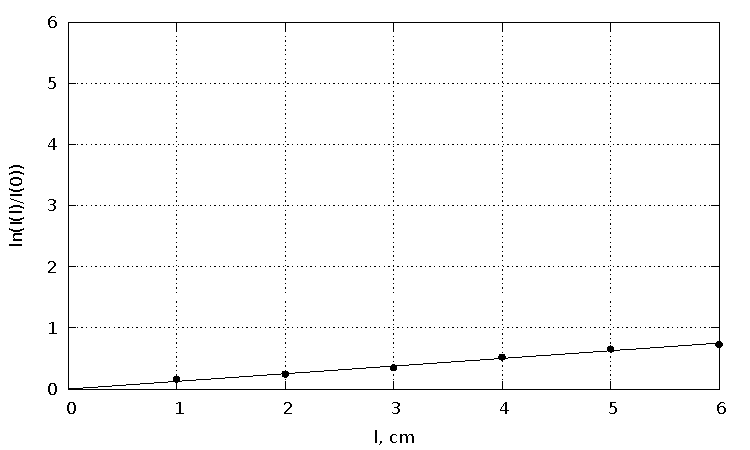
\includegraphics[width=.47\textwidth]{p-0_8}
        \parbox{.47\textwidth}{\caption{При энергии кванта в 0,15 МэВ}} \hfill
        \parbox{.47\textwidth}{\caption{При энергии кванта в 0,8 МэВ}}
    \end{figure}
    
    \emph{Вывод:} провел опыт, моделирующий прохождение гамма-излучения через
    вещество, и исследовал зависимость линейного коэффициента поглощения от
    материала среды, через которую проходит пучок, а также энергии налетающего
    гамма-кванта.
\end{document}
